\chapter{Introduction}
\label{ch:introduction}
%TODO in each section mention research gaps

\section{Tropical forest}
\label{sec:tropical_forest}

	\begin{figure}[ht]
		\centering
		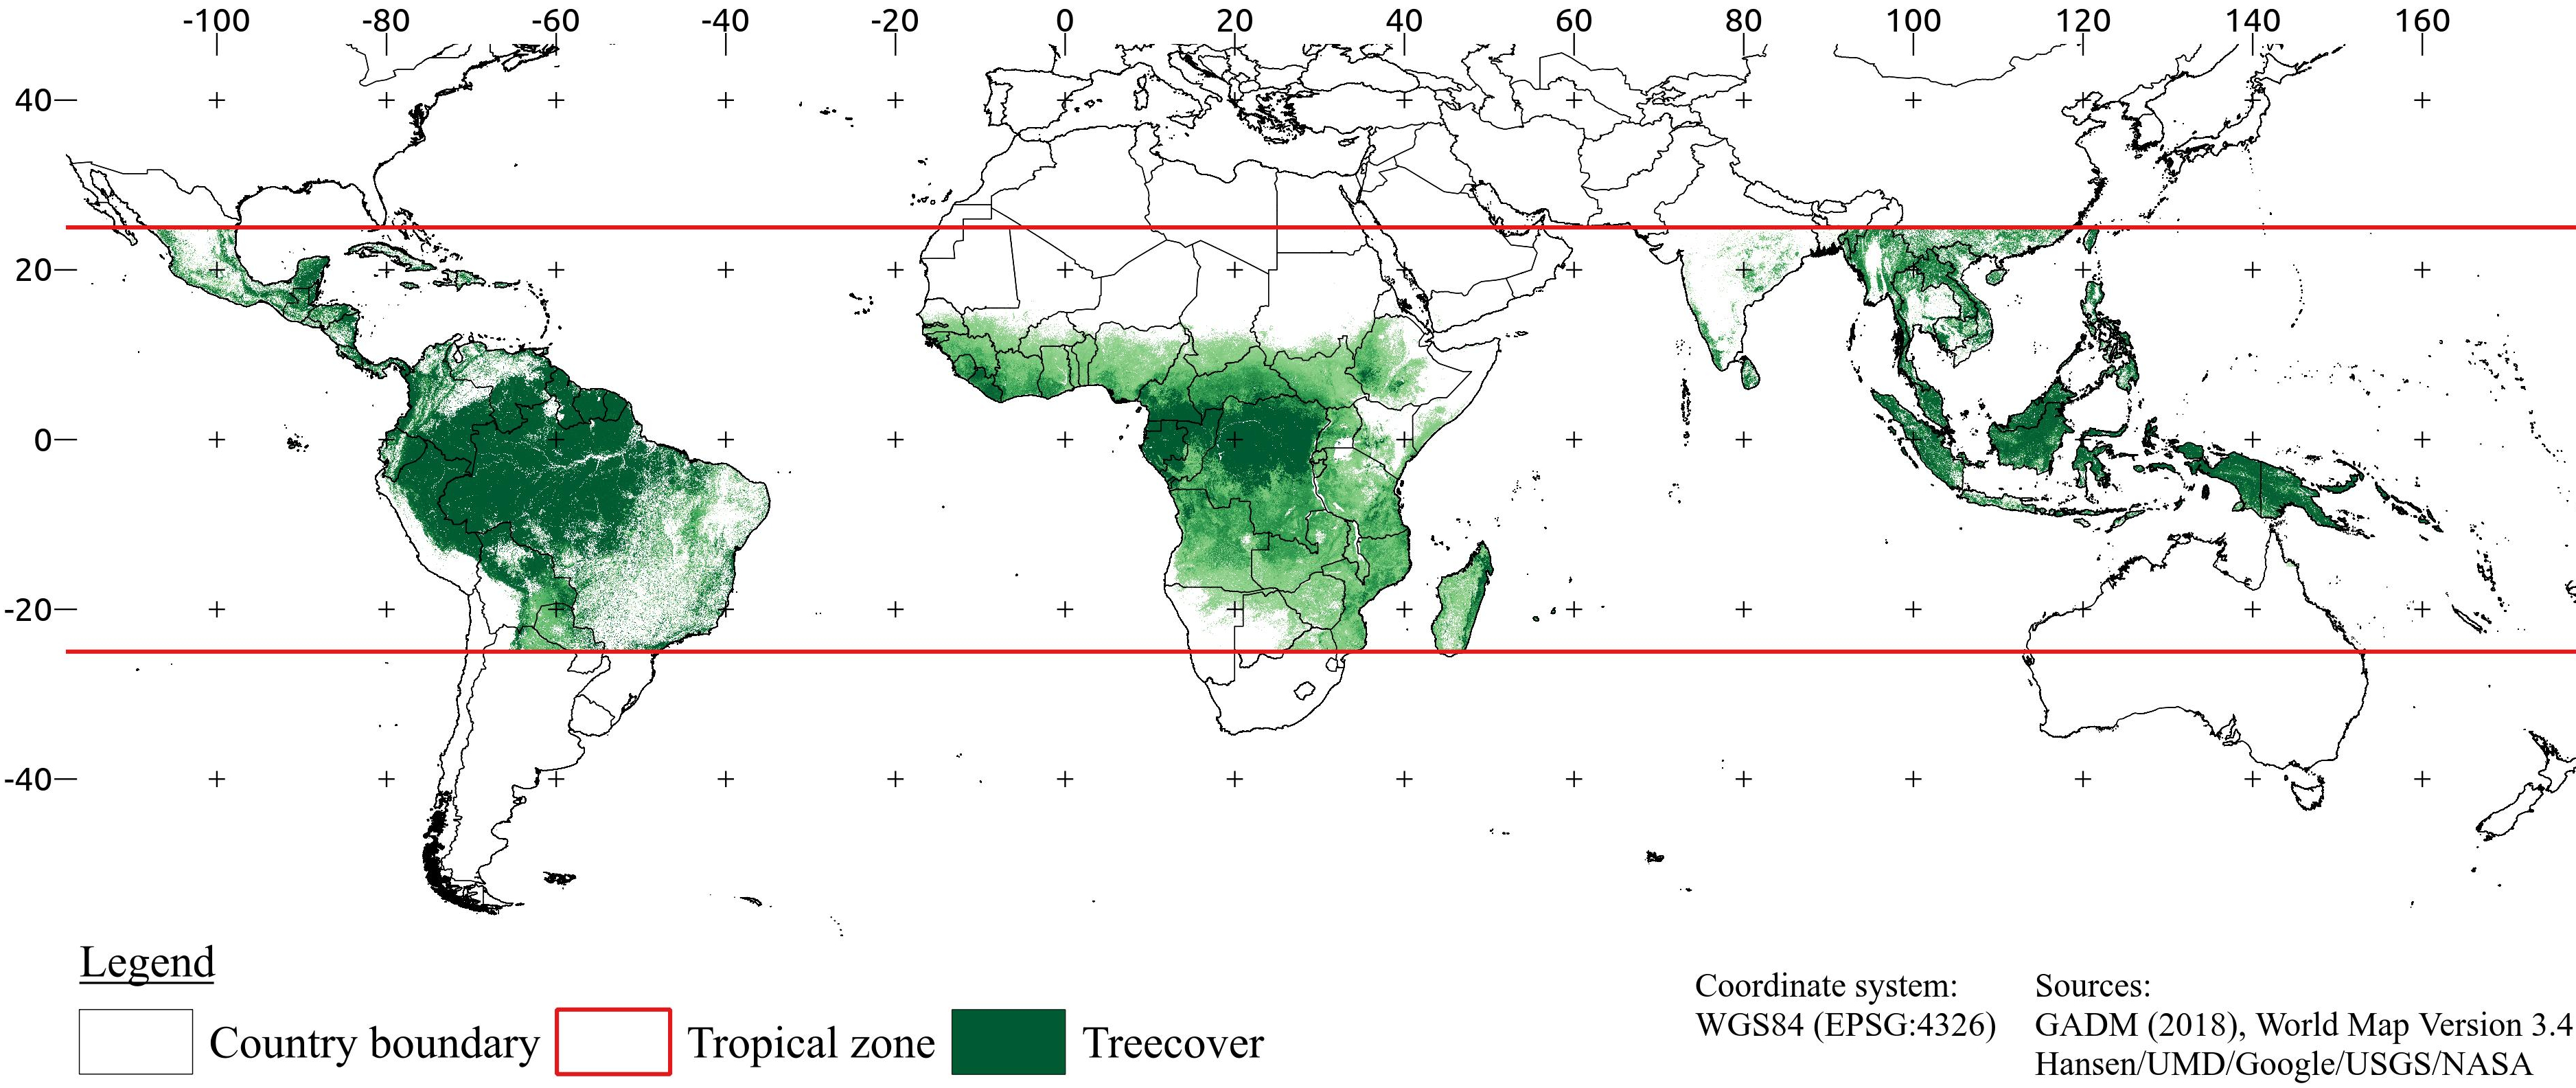
\includegraphics[scale=0.97]{img/intro_overview_frameless}
		\caption[Tropical zone]{Geographic tropical zone framed red and the tropical forest}
		\label{fig:tropicalzone}
	\end{figure}

	\subsection{Current state}
		\lipsum[1-2]
	\subsection{Contribution to climate}
		\lipsum[1-2]
	\subsection{Forest definitions}
		\lipsum[1-3]

\section{Deforestation}
\label{sec:deforestation}
%TODO add spacing between images, add alphanumeric chars to img
%TODO gaps no spatial explicit knowledge on direct drivers
%TODO gaps contribution of deforestation drivers to ghg emissions
%TODO gaps soil organic carbon emissions

	\begin{figure}[ht]
		\centering
		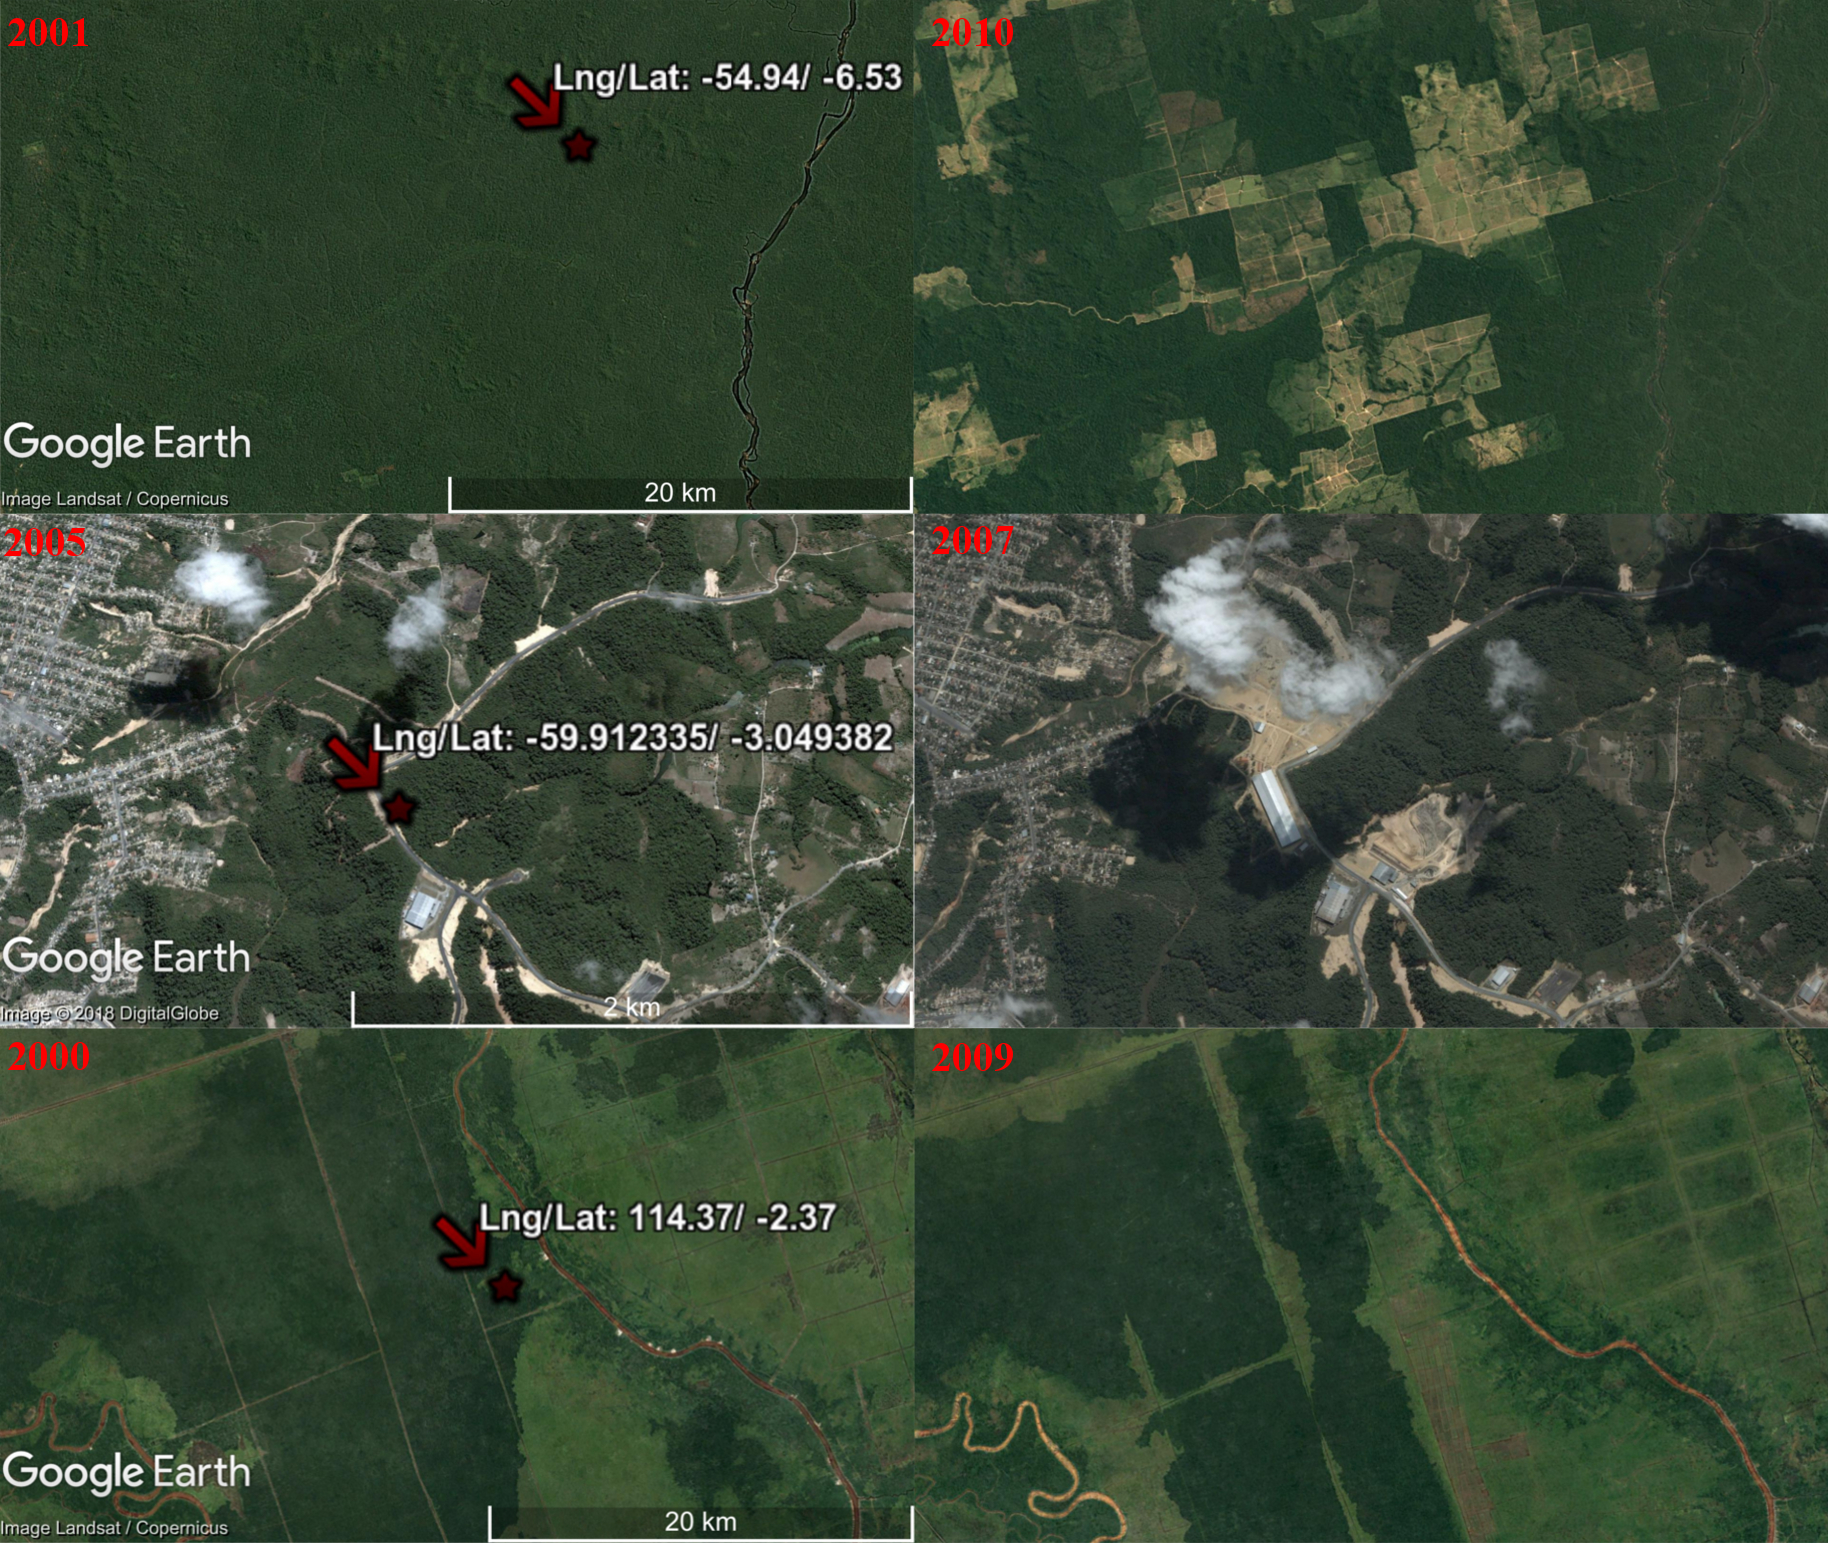
\includegraphics[scale=0.6]{img/deforestation_examples}
		\caption[Deforestation examples]{Upper Brazil agriculture, middle Brazil urbanization, lower Indonesia large scale palm oil plantations}
		\label{fig:deforestationexamples}
	\end{figure}

	\subsection{Land use and land cover change}
		\lipsum[1-2]
	\subsection{Drivers of deforestation}
		\lipsum[1-2]
	\subsection{Emissions trough deforestation}
		\lipsum[1-2]
	\subsection{Removal of AGB}
		\lipsum[1-2]
	\subsection{Soil organic carbon change and soil dynamics}
		\lipsum[1-2]

\section{Ecosystem services}
\label{sec:ecosystem_services}
%TODO gaps no balance for esv

	\subsection{Ecosystem service values}
		\lipsum[1-2]
	\subsection{Research objective and questions}
		\lipsum[1-2]
